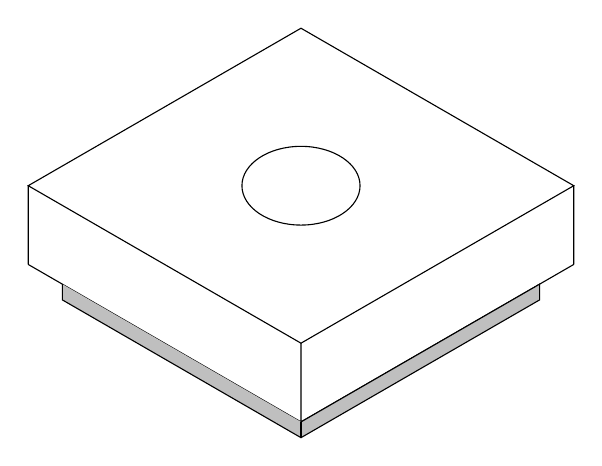
\begin{tikzpicture}
%top
\draw (0,0) -- ++ (30:4) -- ++  (150:4) -- ++ (210:4) -- cycle;
%circle
\draw (0,2) circle [x radius=0.75, y radius=0.5];

%edges
\draw (0,0) -- ++ (0,-1) coordinate (middle)
(0,0) ++ (30:4) -- ++ (0,-1) coordinate (left)
(0,0) ++ (150:4) -- ++ (0,-1) coordinate (right)
(left) -- (middle) -- (right);


%sample
\draw [fill = lightgray]
(0,-1) -- ++ (30:3.5) -- ++ (0,-0.2) -- ++ (210:3.5) -- ++ (150:3.5) -- ++ (0,.2);
\draw (0,-1) -- (0,-1.2);
\end{tikzpicture}